\documentclass[10pt,aspectratio=169]{beamer}

\usetheme[progressbar=frametitle]{metropolis}
\usefonttheme{professionalfonts} 

\usepackage{appendixnumberbeamer}
\usepackage{amsmath}
\usepackage{bbm}
\usepackage[style=apa]{biblatex}
\addbibresource{paper/BibTeX_Library.bib}

\usepackage{booktabs}
\newcommand{\tabitem}{~~\llap{\textbullet}~~}
\usepackage[scale=2]{ccicons}

\usepackage{pgfplots}
\usepgfplotslibrary{dateplot}
\usepackage{tikz}
\usetikzlibrary{decorations.pathreplacing,calc,tikzmark}
\usepackage{graphicx}

\usepackage{animate}
\usepackage{hyperref}
\usepackage{fdsymbol}
\usepackage{multirow}
\usepackage{longtable}
\usepackage{dsfont}

\usepackage[export]{adjustbox}
\tikzset{ffgcaption/.style={%
    anchor=south east,font=\tiny,
    text=white,fill=black,
    fill opacity=.5,text opacity=1,inner sep=2pt,
    text height=1ex,text depth=.25ex}}

% \fullframegraphic 
% renders a single image fullscreen, with an optional credit/caption in the 
% lower right corner.
% Usage: \fullframegraphic[some optional caption]{path/to/image}
% It does not crop the image, but leads to white borders if image does not match
% the aspect ratio of the slide. See commands \fullframegraphicw and
% \fullframegraphich below for cropping alternatives.
\newcommand{\fullframegraphic}[2][]{%
\begin{frame}[plain]%
\begin{tikzpicture}[remember picture,overlay]%
\node[at=(current page.center)] {%
\includegraphics[height=\paperheight,width=\paperwidth,keepaspectratio]{#2}%
};%
\ifx\relax#1\relax\else%
\node[at=(current page.south east),ffgcaption] {#1};%
\fi%
\end{tikzpicture}%
\end{frame}%
}

% \fullframegraphicw: scles image to frame width, cropping excess height.
% use for images that are "taller" than the frame aspect ratio
\newcommand{\fullframegraphicw}[2][]{%
\begin{frame}[plain]%
\begin{tikzpicture}[remember picture,overlay]%
\node[at=(current page.center)] {%
\includegraphics[min height=\paperheight,max width=\paperwidth,keepaspectratio]{#2}%
};%
\ifx\relax#1\relax\else%
\node[at=(current page.south east),ffgcaption] {#1};%
\fi%
\end{tikzpicture}%
\end{frame}%
}

% \fullframegraphich: scales image to frame height, cropping excess width.
% use for images that are wider than the frame aspect ratio
\newcommand{\fullframegraphich}[2][]{%
\begin{frame}[plain]%
\begin{tikzpicture}[remember picture,overlay]%
\node[at=(current page.center)] {%
\includegraphics[max height=\paperheight,min width=\paperwidth,keepaspectratio]{#2}%
};%
\ifx\relax#1\relax\else%
\node[at=(current page.south east),ffgcaption] {#1};%
\fi%
\end{tikzpicture}%
\end{frame}%
}

% \fullframegraphics: more customisable version of fullframegraphic, allowing
% a third argument to insert additional tikz commands for custom overlays.
% use when tooltips or highlights are required on a large image
\newcommand{\fullframegraphics}[3][]{%
\begin{frame}[plain]%
\begin{tikzpicture}[remember picture,overlay]%
\node[at=(current page.center)] {%
\includegraphics[height=\paperheight,width=\paperwidth,keepaspectratio]{#2}%
};%
\ifx\relax#1\relax\else%
\node[at=(current page.south east),ffgcaption] {#1};%
\fi%
#3%
\end{tikzpicture}%
\end{frame}%
}

% Custom command that adds journal abbreviation to cite
\DeclareCiteCommand{\journalcite}
  {\usebibmacro{prenote}} 
  {\printnames{labelname} 
   \setunit{\addcomma\space}
   \printfield{shortjournal} 
   \setunit{\addspace} 
   \printfield{year}}
  {\multicitedelim} 
  {\usebibmacro{postnote}} 

% Custom command that adds journal abbreviation to textcite
\DeclareCiteCommand{\journaltextcite}
  {\usebibmacro{prenote}}
  {\printnames{labelname} 
   (\printfield{shortjournal} 
   \setunit{\addspace} 
   \printfield{year})} 
  {\multicitedelim} 
  {\usebibmacro{postnote}} 

\usepackage{xspace}
\newcommand{\themename}{\textbf{\textsc{metropolis}}\xspace}

\graphicspath{{./presentations/image/}} 

\title{Medical School Environments and Physician Treatment Styles}
\author{Shirley Cai and Ian McCarthy}
\date{\today}
\institute{Emory University\\Department of Economics}
% \titlegraphic{\hfill\includegraphics[height=1.5cm]{logo.pdf}}

\usepackage{textpos}
\addtobeamertemplate{frametitle}{}{%
\begin{textblock*}{10mm}(.88\textwidth,-.8cm)
%\includegraphics[height=0.55cm]{EU_hz_rev.png}
\end{textblock*}}

\begin{document}

\maketitle

% Framing: Fundamental gap in our understanding of how treatment styles develop
\begin{frame}{}

\end{frame}

\begin{frame}{Research question}

\end{frame}

\begin{frame}{This paper}
    \begin{itemize}
        \item 
    \end{itemize}
\end{frame}

\begin{frame}{Literature review}
    
\end{frame}

\begin{frame}{Preview of results}
    Medical school has a lasting impact
        \begin{itemize}
            \item 10pp increase in cath lab availability during training increases later cath rates by 0.58pp
            \item Effect is concentrated among interventional cardiologists
        \end{itemize}

    \vspace{5mm}
    Training imprint does not go away after adjusting for other aspects of training
        \begin{itemize}
            \item Medical school quality
            \item Residency
        \end{itemize}

    \vspace{5mm}
    Compounds into a long-run multiplier of 1.7 when combined with peer effects
\end{frame}

\begin{frame}{Treatment setting}
    \begin{figure}
        \centering
        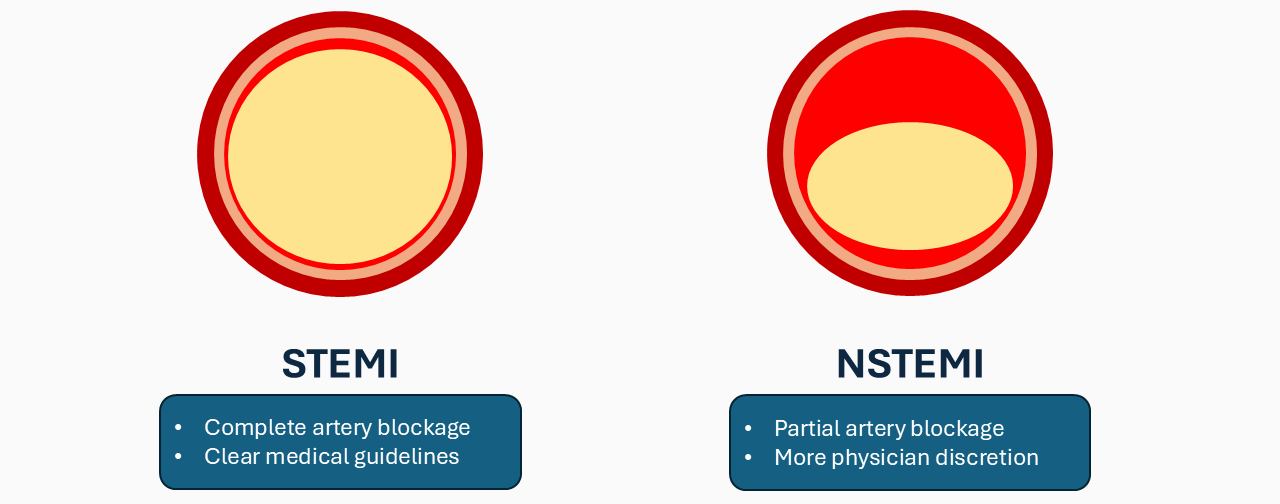
\includegraphics[width=\linewidth]{stemi.png}
    \end{figure}
\end{frame}

% TODO: Revise to make it more along the lines of cath or no cath
\begin{frame}{Treatment setting}
    \begin{figure}
        \centering
        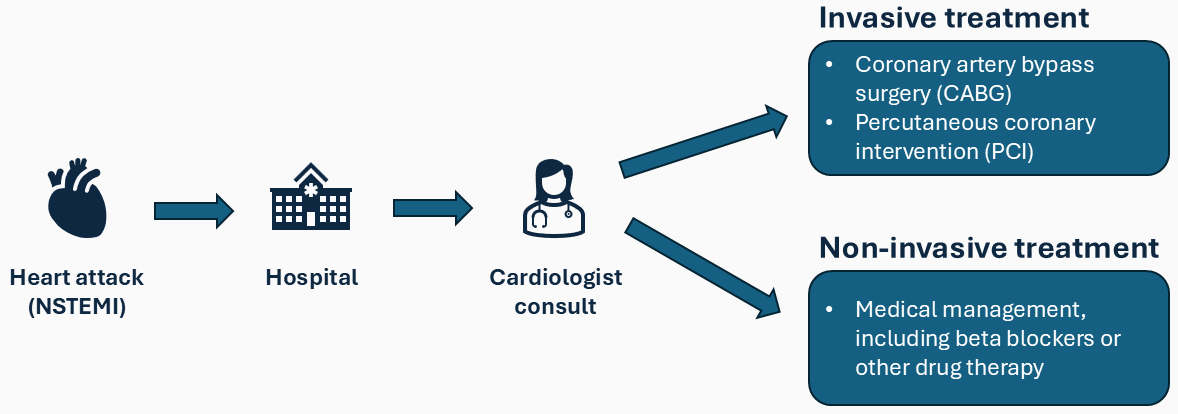
\includegraphics[width=\linewidth]{heart-attack.png}
    \end{figure}
\end{frame}

% TODO: Redo this image. I don't like it much
\begin{frame}{Data: Treatment style}
    Cardiologist cath rate calculated from 100\% FFS Medicare claims (2008-2018)
    \begin{figure}
        \centering
        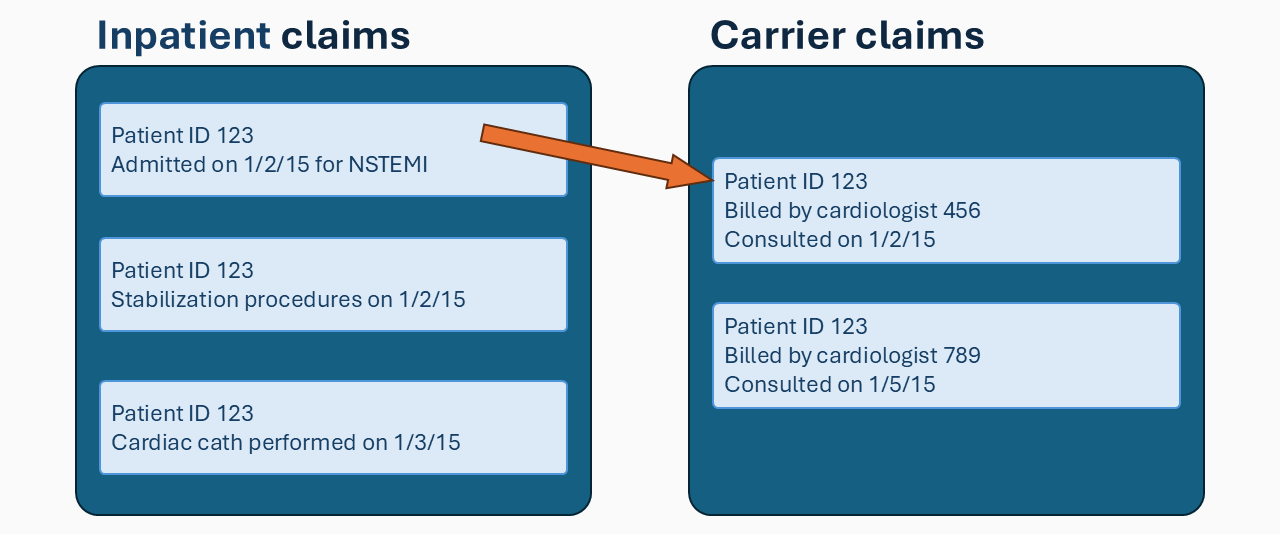
\includegraphics[width=\linewidth]{medicare-claims.png}
    \end{figure}
\end{frame}

\begin{frame}{Data: Treatment style}
    Treatment style = Mean \textbf{residualized cath rate} within two days of admission

    \vspace{10mm}
    Calculate patient-level residual $\varepsilon$ from linear probability model
        \begin{equation*}
            \mathds{1}\{\text{cath}\} = \{\text{Elixhauser comorbitities}\} + \{\text{year FE}\} + \varepsilon
        \end{equation*}
    Aggregate to cardiologist-year level
\end{frame}

% TODO: Can this become a picture
\begin{frame}{Data: Training environment}
    \begin{itemize}
        \item Identify \textbf{medical school and graduation year} from CMS Physician Compare
        \item Map medical school ZIP code to \textbf{HRR} using Dartmouth Atlas crosswalk
        \item Link to \textbf{cath lab data} from AHA Annual Survey
    \end{itemize}

    \vspace{10mm}
    Medical school environment = \textbf{Share of hospitals with a cath lab} in medical school HRR in first year of attendance
\end{frame}

\begin{frame}{Additional data}
    \textbf{On cardiologists}
    \begin{itemize}
        \item MD-PPAS: Specialty, primary practice location
        \item Doximity: Residency and fellowship program, graduation year
    \end{itemize}

    \vspace{5mm}
    \textbf{On medical schools}
    \begin{itemize}
        \item NIH ExPORTER: NIH funding by medical school and year
    \end{itemize}
\end{frame}

\begin{frame}{}
    % Variation over HRR residualized cath rates over time and space
\end{frame}

% Say: We observe the treatment decisions of cardiologists who graduated between 1983 and 2006 for claims billed during 2008 to 2018.

\begin{frame}{Empirical strategy}
    \begin{equation*}
        y_{it} = \beta_\text{train}\tau_i + \theta\bar{y}_{-i,t} + \rho_{m(i)} + \delta_{d(i,t)} + \gamma_t + \epsilon_{it}
    \end{equation*}
    \begin{itemize}
        \item $y_{it}$ = mean residualized cath rate of cardiologist $i$ in year $t$
        \item $\tau_i$ = training-period cath lab share in cardiologist $i$'s medical school HRR
        \item $\bar{y}_{-i,t}$ = leave-one-out mean residualized cath rate of other cardiologists in cardiologist $i$'s practice HRR in year $t$
        \item $\rho_{m(i)}$ = medical school HRR fixed effect
        \item $\delta_{d(i,t)}$ = current practice HRR fixed effect
        \item $\gamma_t$ = year fixed effect
    \end{itemize}
\end{frame}

\begin{frame}{Empirical strategy}
    Using a mover design
        \begin{itemize}
            \item 
        \end{itemize}

    \vspace{10mm}
    \textbf{Identifying variation:} Different cath lab exposure among cardiologists who attended medical school in the same HRR but graduated in different years
    
    \textbf{Identifying assumption:} Within-HRR cath lab adoption is uncorrelated with changes in other cohort-level determinants of practice intensity
\end{frame}

\begin{frame}{Movers vs stayers}
    
\end{frame}

\begin{frame}{Training environment impacts later treatment decisions}
    
\end{frame}

\begin{frame}{Effect is concentrated among interventional cardiologists}
    
\end{frame}

\begin{frame}{Training effect persists after controlling for medical school rank}
    
\end{frame}

\begin{frame}{Training effect persists after controlling for medical school rank}
    
\end{frame}

\begin{frame}{What about residency?}
    
\end{frame}

% TODO: Change slide title. I don't think this is what we are actually saying
\begin{frame}{Can the training effect modify existing variation in treatment style?}
    \begin{equation*}
        \Delta y^{\ast} = \frac{\beta_{\text{train}} \cdot \Delta\tau}{1 - \beta_{\text{dest}}}
    \end{equation*}
\end{frame}

\begin{frame}{Conclusion}
    
\end{frame}

\begin{frame}[standout]
    \Large Thank you! 
    
    \vspace{5mm}
    \small shirley.cai@emory.edu
\end{frame}

\appendix

\begin{frame}{Summary statistics}
    
\end{frame}

%\begin{frame}[allowframebreaks]{References}
%    \printbibliography[heading=none]
%\end{frame}

\end{document}